\chapter{L1's effect on prosodic properties of accented speech}
\label{l1_supraseg}

\section{Introduction}

The previous chapter applies the proposed methodology for accentedness perception to pronunciation based segmental features and proves that integrating L1 pronunciation information by extracting pronunciation score of accented English speech with L1 acoustic model can improve the prediction accuracy of accentedness perception. This chapter will focus on apply the same methodology to speech prosodic features to study whether L1 prosodic patterns affect the perception of accentedness. As mentioned in chapter \ref{sec:methodology}, durational rhythmic features will be used as proxy of speech prosody. The methods and analysis of results are almost the same as chapter \ref{l1_seg}. Details will be introduced in following sections.

\section{Methods}

In chapter \ref{sec:methodology}, the procedure to extract durational rhythmic features is introduced. The extracted rhythmic features for native L1, accented L2 speech and native L2 are represented with $\mathbf{x_{L1}}$, $\mathbf{X_{acc}}$ and $\mathbf{x_{L2}}$ respectively. Note that $\mathbf{x_{L1}}$ and $\mathbf{x_{L2}}$ are vectors because they are the average of features extracted from multiple speech recordings. These three sets of features are converted to accent related features by taking the absolute difference between $\mathbf{x_{L1}}$ and $\mathbf{X_{acc}}$ and $\mathbf{x_{L2}}$ and $\mathbf{X_{acc}}$. $\left| \mathbf{x_{L2}}-\mathbf{X_{acc}} \right|$ represent the difference between the rhythmic patterns of accented speech and target L2 speech while $\left| \mathbf{x_{L1}}- \mathbf{X_{acc}} \right|$ represents the difference between the rhythmic patterns of accented speech and speaker's L1 speech. Here, the subtraction is broadcasted to every row of $\mathbf{X_{acc}}$ to get the contrastive information for each speaker with accent.

The first analysis is the correlation analysis between speech prosodic features and accentedness score averaged of 13 annotators. Similarity, the PCC is calculated between every features of the 18-dimensional feature vectors in a language-dependent way. The procedure is different from previous chapter observing that the feature dimension is higher than pronunciation features, here only the top-12 features with highest PCC with accentedness scores are shown for each language together with the p-values (lower p-value stands for more statistically significant correlation).

Same multiple regression analysis is done here except that the number of input features is changed to 18. Downsampling is not used here since it does not help for German speakers. Thus, for each language, multiple regression analysis is done between 18-dimensional speech rhythmic measurements and accentedness  scores of 30 speakers. Specifically, $\left| \mathbf{x_{L2}}-\mathbf{X_{acc}} \right|$ is used as the baseline model which on takes the difference of speech rhythmic patterns between accented speech and L2 into consideration. Then, $\left| \mathbf{x_{L1}}- \mathbf{X_{acc}} \right|$ can be combined into the baseline feature set to model the distance between accented speech and L1 on suprasegmental feature space. Finally, input to the baseline model is a 18-dimensional feature vector while input to the proposed model is a 36-dimensional feature vector.

As in chapter \ref{l1_seg}, the input feature vectors are first normalized with mean and standard deviation on each dimension. Then, a feature selector based on univariate regression test is applied to select the most predictable features. Ridge regression is used to learn the relationship between input features and accentedness score. The same leave-one-speaker-out CV is employed to evaluate the performance on accentedness prediction. Hyperparameters including number of features selected and strength of 2-norm regularization in ridge regression are tuned to achieve the best CV performance. PCC and MAE are reported language dependently. To better illustrate the process, figure \ref{fig:l1_supraseg_diagram} shows the whole procedure of multiple regression analysis.

\begin{figure}[t]
        \begin{minipage}[t]{1.0\linewidth}
        \centering
            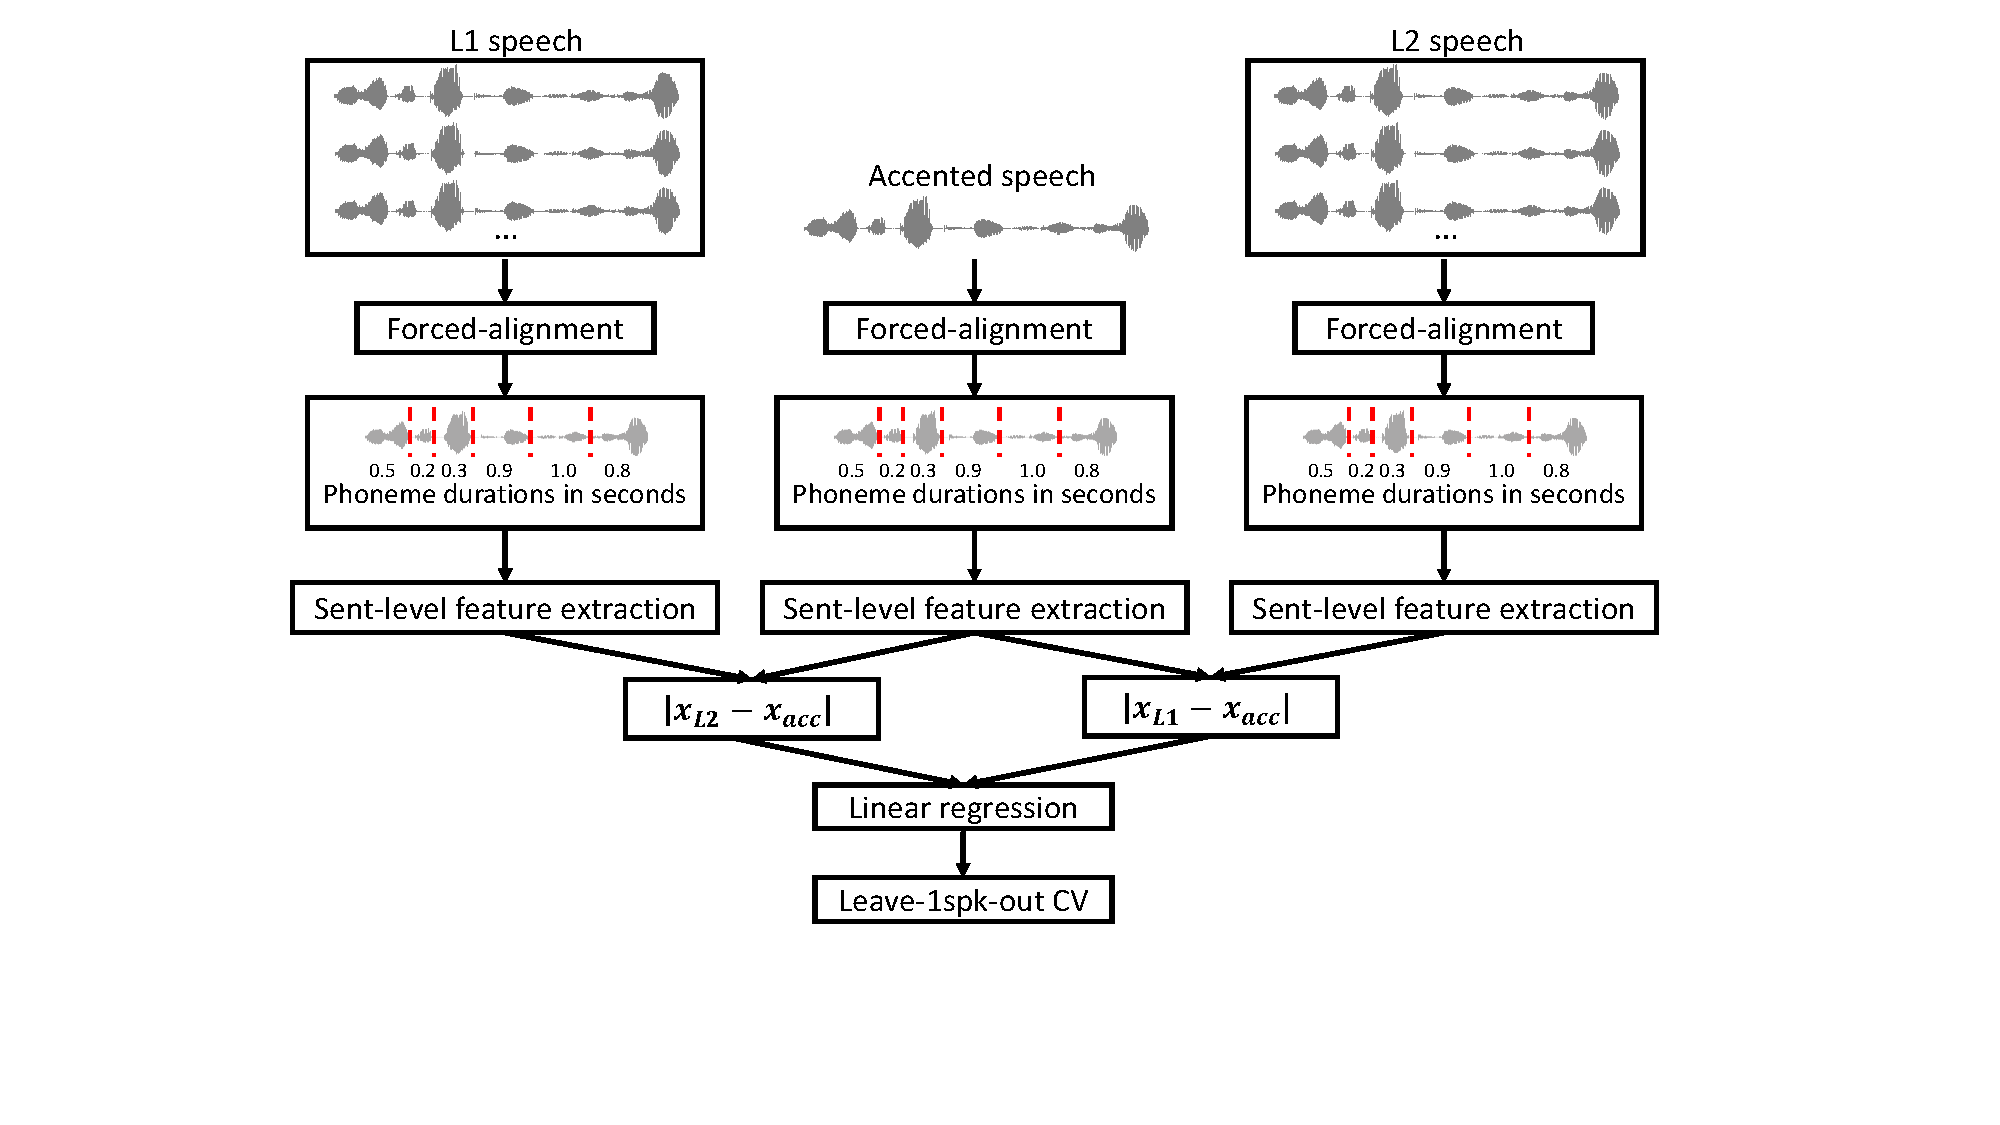
\includegraphics[width=5.0in]{figures/method_diagram_supraseg.pdf}
        \end{minipage}%
        \caption{Diagram of the procedure for multiple regression analysis between suprasegmental prosodic features and accentedness scores. Here, $\mathbf{x_{L1}}$ and $\mathbf{x_{L2}}$ are the average of features of all speech recordings. $\mathbf{x_{acc}}$ is the feature vector for one accented speech recording.}
        \centering
        \label{fig:l1_supraseg_diagram}
     \end{figure}

\section{Results}
\subsection{Results of correlation analysis}

\begin{figure}[]
        \begin{minipage}[t]{0.5\linewidth}
        \centering
            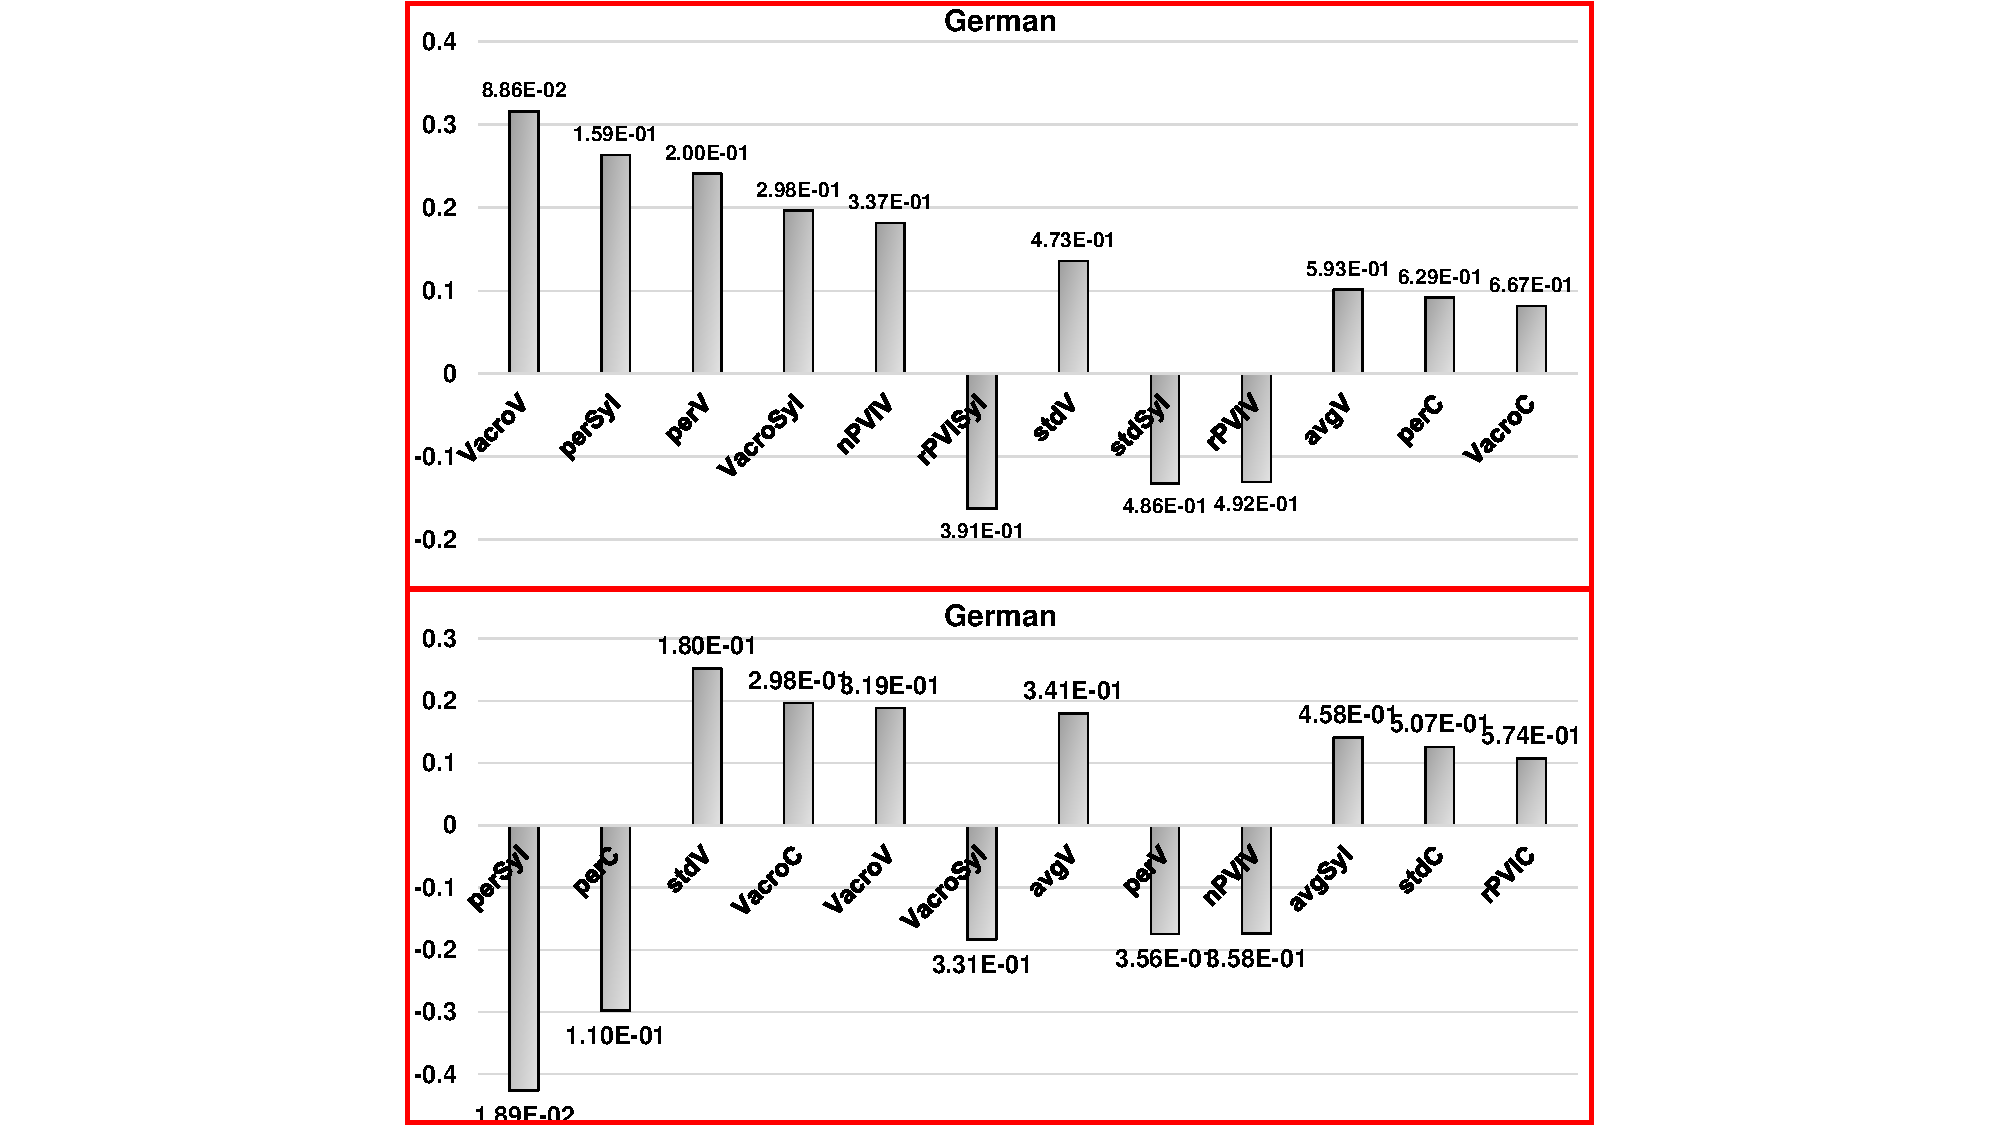
\includegraphics[width=3in]{figures/supra_seg_bar_plot/german.pdf}
        \end{minipage}%
        \begin{minipage}[t]{0.5\linewidth}
        \centering
            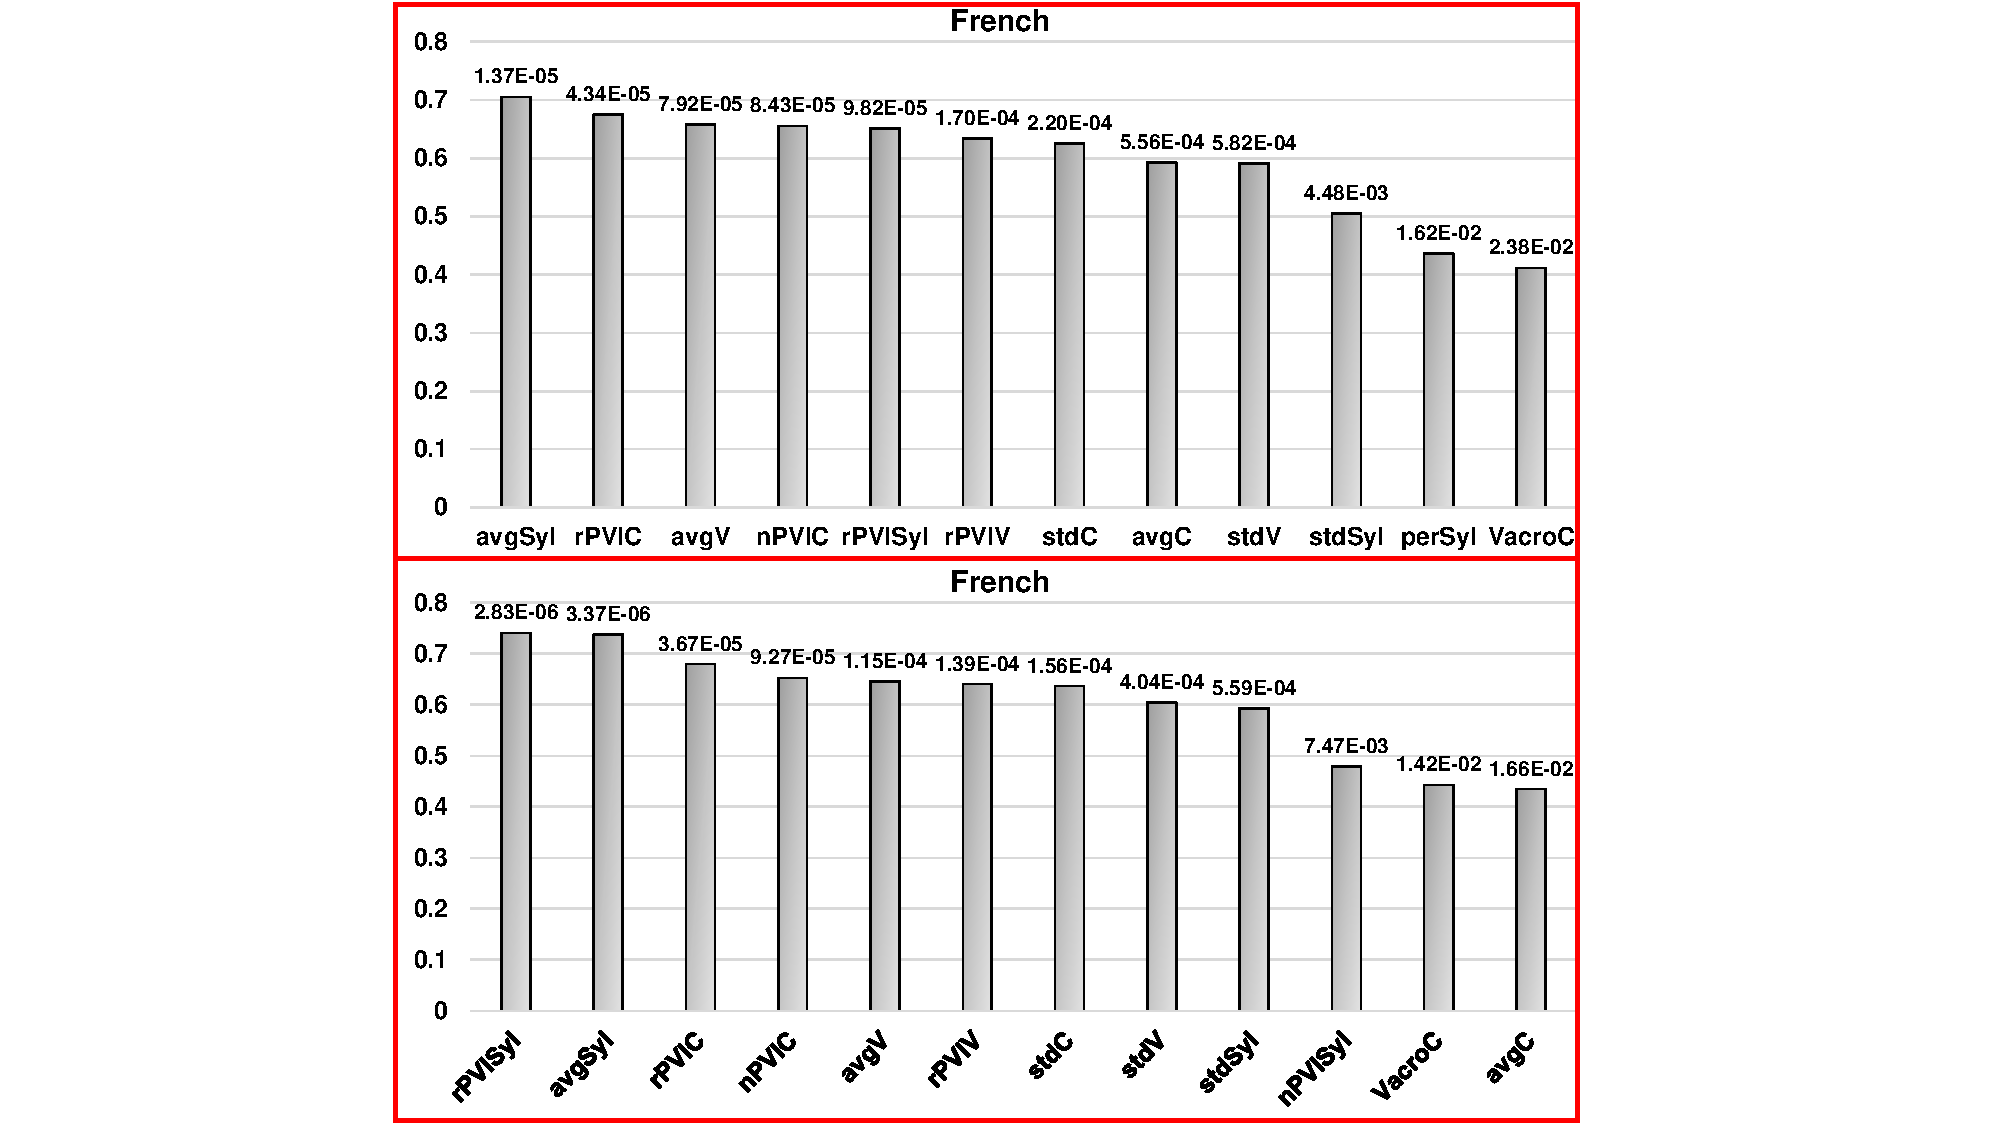
\includegraphics[width=3in]{figures/supra_seg_bar_plot/french.pdf}
        \end{minipage}%
        \\
        \begin{minipage}[t]{0.5\linewidth}
        \centering
            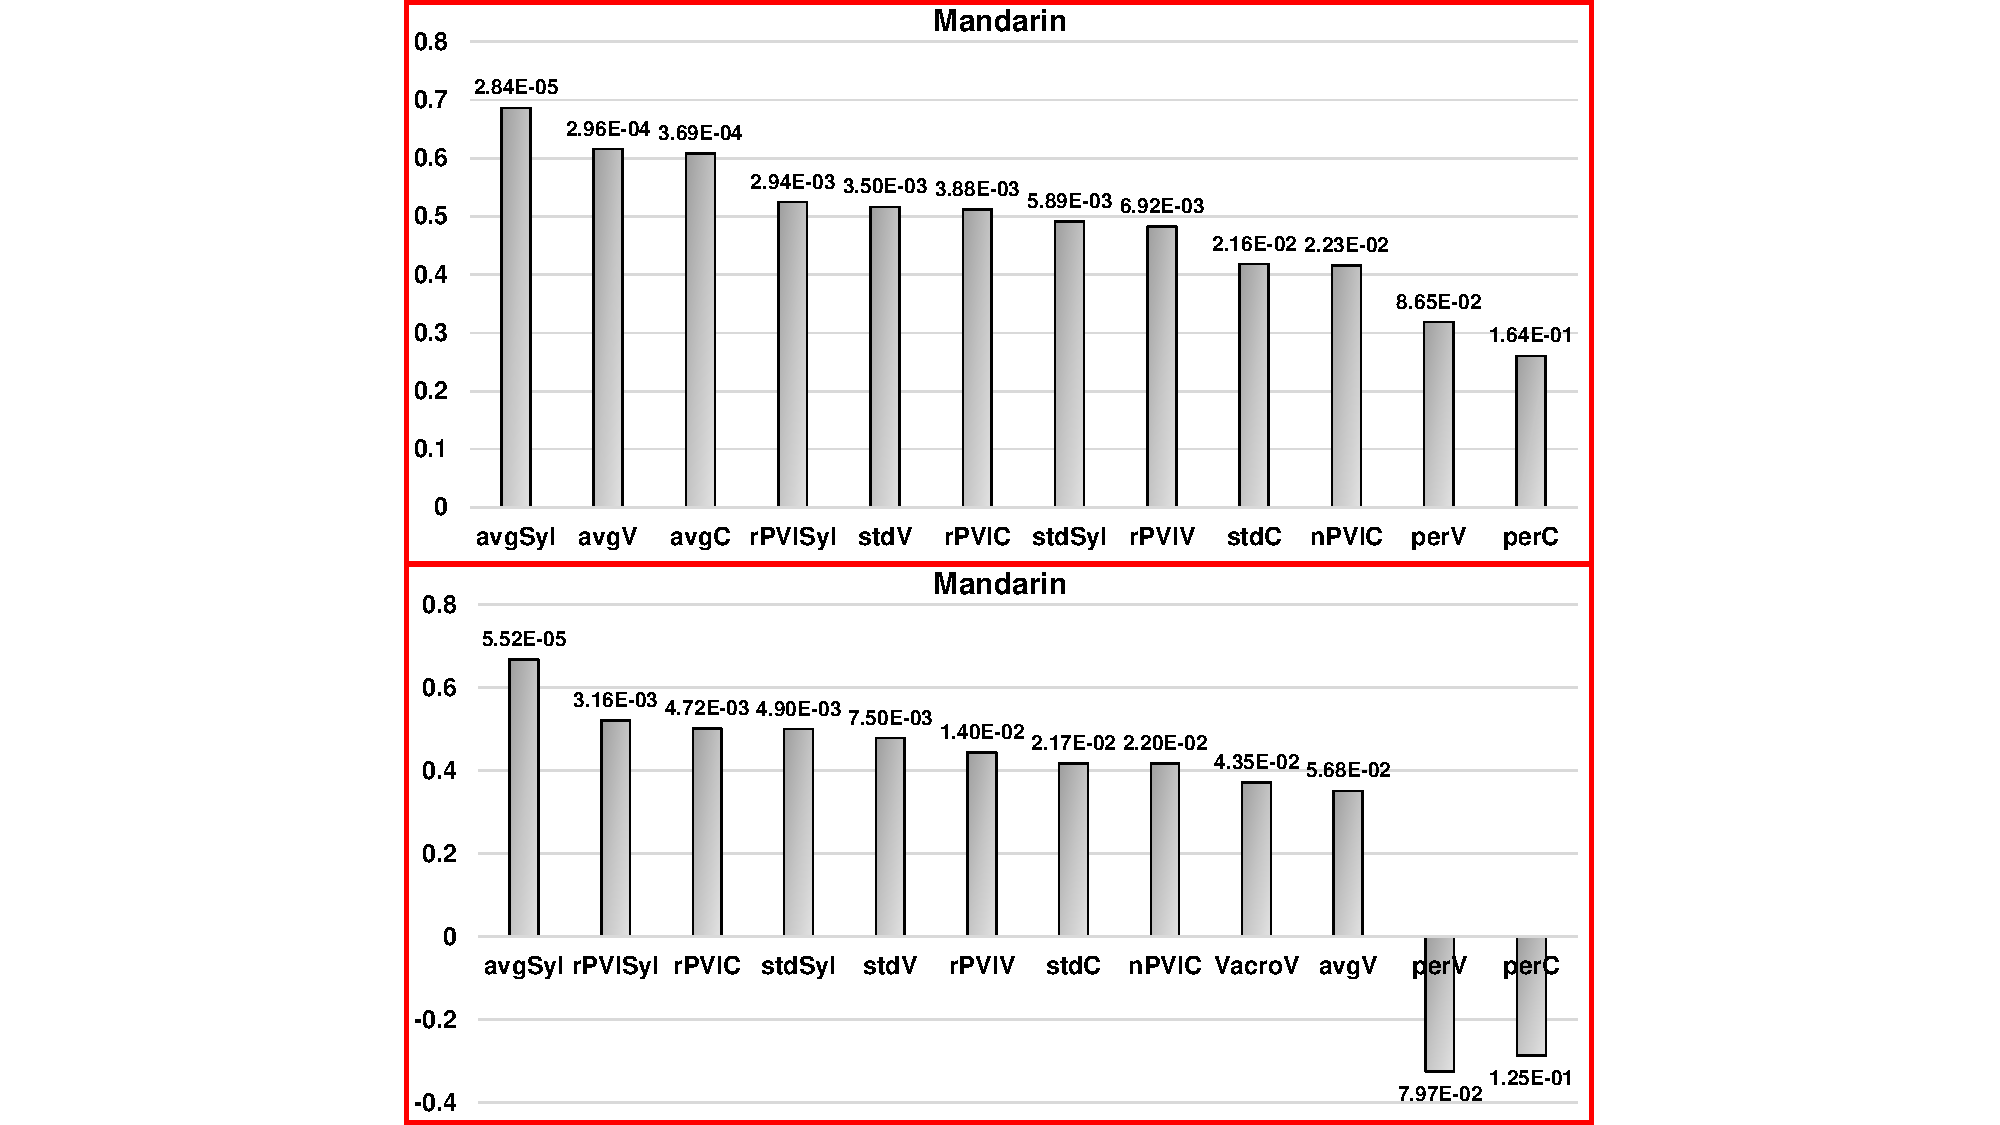
\includegraphics[width=3in]{figures/supra_seg_bar_plot/mandarin.pdf}
        \end{minipage}%
        \begin{minipage}[t]{0.5\linewidth}
        \centering
            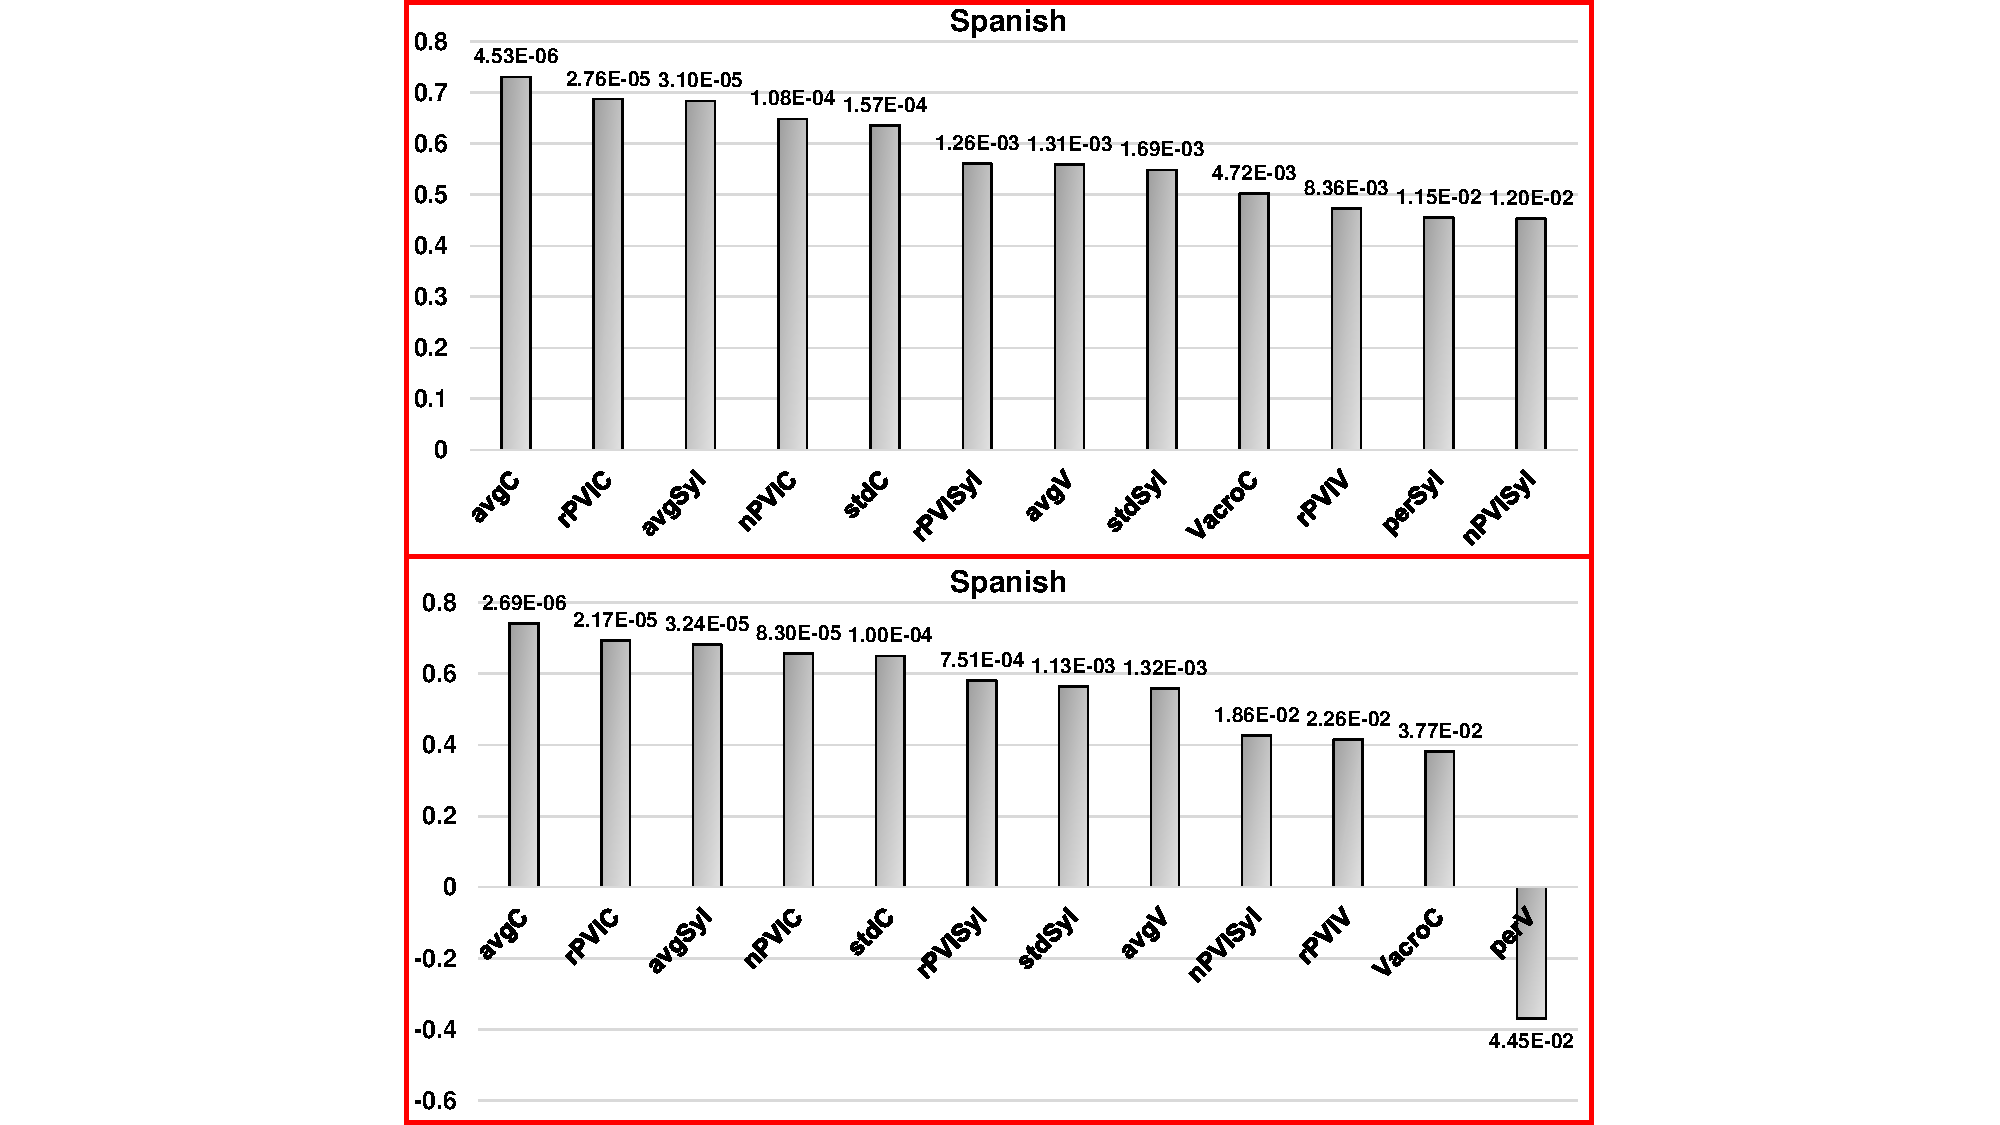
\includegraphics[width=3in]{figures/supra_seg_bar_plot/spanish.pdf}
        \end{minipage}%
        \caption{Bar plots of the top-12 features highly correlated with accentedness scores in feature sets $\left| \mathbf{x_{L2}}-\mathbf{X_{acc}} \right|$ (upper panel in each subfigure) and $\left| \mathbf{x_{L1}}- \mathbf{X_{acc}} \right|$ (lower panel in each subfigure). Y-axis is the correlation coefficients with accentedness score and X-axis is feature names. The numbers on top of each bar are the p-value for testing non-correlation.}
        \centering
        \label{fig:supraseg_bar}
     \end{figure}

In figure \ref{fig:supraseg_bar}, PCC together with p-value between two sets of speech rhythmic features and accentedness scores of four different foreign languages are presented. Feature names on X-axis are abbreviations: per\{V,C,Syl\} represents the percentage of durations of vowels, consonants and syllables, avg\{V,C,Syl\} represents the average durations, std\{V,C,Syl\} represents the standard deviation of durations, Vacro\{V,C,Syl\} represents the mean-normalizd standard deviation of durations, rPVI\{V,C,Syl\} represents the Raw PVI of durations and nPVI\{V,C,Syl\} represents the Normalized PVI) of durations. From the figure, there are several interesting observations:

\begin{enumerate}
\item Except for German speakers, other three languages all have relatively high correlation coefficients ($>$0.6) with accentedness scores. This can be attributed to the similarity of rhythmic patterns between English and German (as shown in figure \ref{fig:rhythmic_mds} and table \ref{table:conf_rhythmic}, also in the study by \cite{li2014l2}). It becomes hard to use rhythmic features to differentiate between mild and strong accent when the rhythmic patterns of L1 is already very close to L2.
\item As shown in previous chapter, the most predictable features extracted with L1 acoustic models have opposite correlation with accentedness scores compared to features extracted with L2 acoustic models. However, for rhythmic features, it can be found that most features of both $\left| \mathbf{x_{L2}}-\mathbf{X_{acc}} \right|$ and $\left| \mathbf{x_{L1}}- \mathbf{X_{acc}} \right|$ are positively correlated with accentedness scores. Only a few dimensions of $\left| \mathbf{x_{L1}}- \mathbf{X_{acc}} \right|$ have negative correlation with accentedness scores. This indicates that for some speakers, values of feature dimensions in $\mathbf{X_{acc}}$ are not within the range from values of $\mathbf{x_{L2}}$ to values of $\mathbf{x_{L2}}$ in corresponding dimensions while values on some feature dimensions are between the values in L1 and L2. This is also observed in the study by \cite{white2007calibrating}. This observation is consistent with the founds in \citep{li2014l2} where the authors believe that for speech rhythm acquisition there is a multisystemic model of L2 rhythm acquisition and both transferred L1 knowledge and universal effects independent of L1 played a role.
\item For languages that have high correlation coefficients, it can be found that the average durations features and PVI features are the most correlated ones. This is also consistent with studies by \cite{ordin2015acquisition} where they show the different rhythmic feature values in different proficiency levels: beginners, intermediate and advanced although they did not provide correlation coefficients between rhythmic feature values and how strong the accent is.
\end{enumerate}

\subsection{Results of multiple regression analysis}

During the experiment, it was found that For French and Mandarin, using feature set [$\left| \mathbf{x_{L2}}-\mathbf{X_{acc}} \right|$, $\left| \mathbf{x_{L2}}-\mathbf{X_{acc}} \right|$-$\left| \mathbf{x_{L1}}- \mathbf{X_{acc}} \right|$] as the way to integrate L1 information gave the best performance of leave-one-speaker-out CV; for Spanish speaker, feature set [$\left| \mathbf{x_{L2}}-\mathbf{X_{acc}} \right|$, $\left| \mathbf{x_{L1}}- \mathbf{X_{acc}} \right|$] gave the best performance. Since for French and Mandarin, using [$\left| \mathbf{x_{L2}}-\mathbf{X_{acc}} \right|$, $\left| \mathbf{x_{L1}}- \mathbf{X_{acc}} \right|$] can also achieve better performance than the baseline model, the difference of the best feature sets across languages is probably due to different speech prosody patterns.
In table \ref{table:supraseg_pred}, both the PCCs and MAEs between model predicted accentedness and human annotated accentedness for 3 groups of speakers are presented. Here, the results for German speakers are not showed because the prediction of the regression model is pretty bad and has negative correlation with human accentedness scores. Downsampling did not help in this case. This is consistent with the correlation analysis in figure \ref{fig:supraseg_bar}, where German rhythmic features have low correlation with accentedness score. There is no downsampling for French seapekrs either because without downsampling, the performance on French speakers is already satisfied. There is a consistent improvement when adding L1 rhythmic patterns based features for all 3 L1s. These results show that there is an improvement in model performance consistently and across all three languages after adding features from contrastive information with L1 rhythmic patterns. It proves that the rhythmic contrastive information between accented speech and L1 can provide extra information for accentedness prediction. This is also despite the fact that the annotators know little about the acoustic properties of the speakers' L1s.

\begin{table}[]
\centering
\caption{PCCs and MAEs between predicted accentedness and human scores for speakers of three different L1s.}
\label{table:supraseg_pred}
\begin{tabular}{|c|c|c|c|c|}
\hline
 & \multicolumn{2}{c|}{[$\left| \mathbf{x_{L2}}-\mathbf{X_{acc}} \right|$]} & \multicolumn{2}{c|}{With $\left| \mathbf{x_{L1}}- \mathbf{X_{acc}} \right|$} \\ \hline
 & PCC & MAE & PCC & MAE \\ \hline
French & 0.647 & 0.310 & 0.680 & 0.289 \\ \hline
Mandarin & 0.581 & 0.425 & 0.712 & 0.380 \\ \hline
Spanish & 0.698 & 0.507 & 0.729 & 0.482 \\ \hline
\end{tabular}
\end{table}

\begin{table}[]
\centering
\caption{Selected feature dimensions from [$\left| \mathbf{x_{L2}}-\mathbf{X_{acc}} \right|$, $\left| \mathbf{x_{L2}}-\mathbf{X_{acc}} \right|$-$\left| \mathbf{x_{L1}}- \mathbf{X_{acc}} \right|$] for French and Mandarin speakers or [$\left| \mathbf{x_{L2}}-\mathbf{X_{acc}} \right|$, $\left| \mathbf{x_{L1}}- \mathbf{X_{acc}} \right|$] for Spanish speakers. ``num\_feature'' stands for the total number of selected features by feature selection.}
\label{table:supraseg_feat_sel}
\begin{tabular}{|c|c|l|l|l|}
\hline
 & \multicolumn{4}{c|}{Selected feature dimensions} \\ \hline
\begin{tabular}[c]{@{}c@{}}French \\ (num\_feat=25)\end{tabular} & \multicolumn{4}{c|}{\begin{tabular}[c]{@{}c@{}}avgC, avgSyl, stdC, stdSyl,VacroC, \\ perC, perSyl, rPVIC, rPVISyl, nPVISyl\end{tabular}} \\ \hline
\begin{tabular}[c]{@{}c@{}}Mandarin \\ (num\_feat=15)\end{tabular} & \multicolumn{4}{c|}{avgV, avgC, stdV,perV} \\ \hline
\begin{tabular}[c]{@{}c@{}}Spanish \\ (num\_feat=11)\end{tabular} & \multicolumn{4}{c|}{avgC, avgSyl, stdC, rPVIC, rPVISyl,nPVIC} \\ \hline
\end{tabular}
\end{table}

In order to show that features extracted with L1 rhythmic patterns really helps with predicting accentedness scores, in table \ref{table:supraseg_feat_sel}, L1 rhythmic patterns based features that are selected to predict accentedness scores are showed. Since the multiple regression analyses are done language-independently, different sets of features are selected for different languages, and the number of features selected for each language is also presented in the table. It can be found that for French and Spanish speakers, the durational measurements of L1 consonants and syllables are more import features while for Mandarin speakers the durational measurements of L1 vowels are more import features. The study by \cite{li2014l2} compared durational measurements of Mandarin accented English and native English. They showed that vocalic rhythmic measurements can well discriminate Mandarin learners at different proficiency levels. While for French and Spanish speakers, there are no studies showing the progressive change of consonantal and syllable rhythmic measurements along the proficiency level. The results here are reasonable considering both French and Spanish are syllable-timed languages while English is stress-timed languages. The results of the multiple regression analysis further validate the hypothesis in chapter \ref{introduction} that ``If this distance information is added to the feature sets for automatic accentedness evaluation, the performance will be improved.

\section{Discussion}

This chapter shows that the speech prosodic properties transferred from L1 can also help deciding how strong the foreign accent is for L2 learners. This conforms with previous studies where they show the L1 effect in L2 prosody acquisition \citep{rasier2007prosodic,stockmal2005measures,white2007calibrating,li2014l2,ordin2015acquisition}. However, based on the correlation analysis in figure \ref{fig:supraseg_bar}, on most feature dimensions, it does not indicate that if the rhythmic property on that dimension is further from L1, the foreign accent is milder. This is in contrast to the results in table \ref{table:seg_corr}. The first possible reason is that while previous studies show the effect of L1 on L2 rhythmic pattern acquisition, there are also obvious universal effect that are independent of L1. For example, the study \cite{ordin2015acquisition} showed that the PVI measurements of English speech produced by French speakers can be even higher than native English speakers given that English speech has much higher PVI measurements than French speech. The second possible reason is that all the rhythmic measurements in this study are based on automatic forced alignment. For speakers with not very strong accent, the will be much less forced-alignment errors. However, for speakers with very strong accent, the forced-alignment results may not be that accurate. This will also affect the correlation analysis between features and accentedness scores. Another interesting observation is that for German speakers, rhythmic features do not help in predicting accentedness score. This is due to the similarity between English and German rhythmic patterns. Both perceptually and computationally, it is hard to find useful rhythmic features extracted from acoustic signal that can discriminate different degrees of foreign accent.

Compared to the results in chapter \ref{l1_seg}, for German and Mandarin speakers, using only segmental pronunciation based features can better predict accentedness scores than using only supra-segmental rhythmic features; while for French and Spanish, the supra-segmental rhythmic features perform better. Compared to previous studies using phonological properties transplantation to investigate the relative importance of segmental and supra-segmental in accentedness perception, this study provide a new way to look at the same problem with the advantage that this method can provide quantitative analysis.
 